\documentclass[11pt]{article}
\usepackage[a4paper,margin=2.5cm]{geometry}
\usepackage{graphicx}
\usepackage{booktabs}
\usepackage{amsmath,amssymb}
\usepackage[hidelinks]{hyperref}
\graphicspath{{../data/}}
\newcommand{\Tobs}{T_{\rm obs}}
\newcommand{\psig}{p_{\rm sig}}
\newcommand{\pnull}{p_{\rm null}}

\title{A forward test of the circumbinary-accretion model of the periodic quasar SDSS~J025214.67$-$002813.7 on ZTF data from 2020 to 2025}
\author{Qianghao Wu}
\date{28 November 2026}

\begin{document}
\maketitle

\begin{abstract}
\noindent Liao et al.\ (2021) reported a 4.4-yr periodicity in the optical light curves of the quasar SDSS J025214.67$-$002813.7 (J0252) and found that a bursty circumbinary-accretion model (mass ratio $q = 0.11$) fits them best. Their r-band fit has a period of 1466~d, and their data end in early 2019. We continued their plotted r-band model in phase at 1466~d and compared it with the public ZTF r-band data from July 2020 to October 2025 (97 detections, about 1.3 cycles). We wrote down the test before we compared the data with the model. The fitted amplitude of the continued curve is $T = -0.66$, where the forecast predicts $T = 1$ and no relation gives $T = 0$. So the data run in anti-phase with the continuation. The quasar is near the ZTF detection limit, and the first noise model did not include this. A post hoc addendum, written before its computation, added detection censoring and the damped-random-walk parameters that Liao et al.\ published. In this model, if the forecast is true, the probability of $T \le -0.66$ is 0.0005 at their best-fit noise parameters and at most 0.002 in their 68\% region. Nearby ZTF objects show 1.7 to 2.1 times more scatter in $T$ than the model gives. After this calibration the probability is 0.01 to 0.04, which is above the registered threshold of 0.01. So the data disfavour the continuation but do not refute it. The test has low power (about 0.3). Post hoc, continuations at 1604 and 1607~d, inside the period ranges of Liao et al., give a positive $T$. The result does not test the 4.4-yr periodicity as such. This work has not yet been reviewed by experts. The computations and the text were produced by AI models (from Anthropic and OpenAI), working under the author's direction.
\end{abstract}

\section{Introduction}

A pair of supermassive black holes in a close orbit can change the accretion rate of the gas around it with the orbital period. A quasar with periodic brightness changes is therefore a candidate binary. Normal quasars also vary at random. Their variability is red noise, which a damped random walk (DRW) describes well \cite{kelly2009}. A few cycles of red noise can look periodic, so a period in a short light curve is weak evidence \cite{vaughan2016}. A real period continues after the data that found it. A chance pattern does not.

Chen et al.\ (2020) searched 625 quasars with Dark Energy Survey (DES) and Sloan Digital Sky Survey (SDSS) light curves for periodic variability \cite{chen2020}. Liao et al.\ (2021) then studied one of its candidates, SDSS J025214.67$-$002813.7 (J0252, redshift 1.53) \cite{liao2021}. They wrote: ``Here we report discovery of a periodicity ($P$=1607$\pm$7 days) at 99.95\% significance [\dots] in the optical light curves of a redshift 1.53 quasar [\dots] The light curves are best fit by a bursty model predicted by hydrodynamic simulations of circumbinary accretion disks.'' Their Table~2 gives the period of the bursty $q=0.11$ model for each band: 1511 (g), 1466$^{+64}_{-12}$ (r), 1506 (i), 1562$^{+248}_{-99}$ (z) and 1476$^{+128}_{-5}$~d (joint griz fit). The Lomb--Scargle periods are 1607 to 1632~d. Their data end in early 2019. In their Section~6 they wrote: ``The significance of a real periodicity should increase as more cycles are covered.''

Later work on J0252 used the same data. Foord et al.\ (2022) studied its X-ray emission and its spectral energy distribution and found an X-ray spectrum consistent with that of a single active nucleus \cite{foord2022}. Covino, Tobar and Treves (2022) reanalysed the light curves with Gaussian processes and concluded that ``the possibility that this is a chance result cannot be ruled out'' \cite{covino2022}. We found no test of J0252 on data taken after the paper. The search covered the citing works of both papers, two archives of AI-produced results, and the web (Section~\ref{sec:prior}).

Other candidates were tested in similar ways. Rigamonti et al.\ (2025) reanalysed the light curves of SDSS J2320+0024 and found no significant evidence for a periodic signal over red noise \cite{rigamonti2025}. El-Badry, Hogg and Rix (2026) tested whether the periodic signals of 181 Gaia DR3 candidates continue in later ZTF data. In all 116 cases with ZTF data, the periodic model failed to predict the later variability \cite{elbadry2026}. A previous result of ours tested the 86 ZTF candidates of Chen et al.\ (2024) \cite{chen2024} on later ZTF data and found no predictive periodicity \cite{wu2026}. None of these tests uses J0252.

This paper gives a forward test of the bursty-model fit of J0252. We take the r-band model curve that Liao et al.\ plotted, continue it in phase at their r-band period, and compare it with public ZTF r-band data from 2020 to 2025. The test is narrow. It concerns one continuation of one fit. It does not test the 4.4-yr period in general (Section~\ref{sec:scope}).

\section{Data}

\paragraph{The model curve.} Figure~1 of Liao et al.\ shows the r-band data and, as a thick curve, the best-fit $q = 0.11$ bursty model with a red-noise background. The figure is a raster image inside a PDF file of the arXiv source (arXiv:2008.12317v3). We digitized the thick curve from MJD 50909 to 58889 by its colour (\texttt{checks/digitize\_model.py}). The digitization error is about 0.01 to 0.04~mag. Plot markers of the same colour contaminate the curve near MJD 53700 and 58400--58500. The model curve is a scaled simulation curve. It is not strictly periodic: the spacings of its troughs are about 1350 to 1650~d.

\paragraph{The template.} We folded the digitized curve at $P = 1466$~d, took the median in 50 phase bins and removed the mean. The template has a peak-to-peak range of 0.33~mag. The forecast for a time $t$ after the cutoff is the template at the phase of $t$. This continuation is our construction. Liao et al.\ give no forecast curve after MJD 58889.

\paragraph{ZTF data.} We downloaded the ZTF light curves from the NASA/IPAC Infrared Science Archive (IRSA) \cite{bellm2019,masci2019} in a 2.2-arcsec circle around the quasar. The held-out sample is all zr points with \texttt{catflags} $= 0$ and MJD $> 58927$ (2020-03-19). The data of Liao et al.\ and their plotted model curve (to MJD 58889) end before this cutoff. The sample has 97 points from MJD 59061 to 60968 (2020-07-31 to 2025-10-20), on two ZTF objects (91 points in field 402 and 6 in field 1446). This is about 1.3 cycles of the continuation. For the censored model (Section~\ref{sec:censored}) we also downloaded a 0.08-degree zr cone. It gives 345 good exposures of the two CCD quadrants that contain the quasar after the cutoff (312 and 33). ZTF lists the quasar on 97 of them (28\%).

\section{Method}

\subsection{Test statistic}
For each listed point $i$ we fit
\begin{equation}
m_i = c_{{\rm obj}(i)} + T\,x(t_i) + \varepsilon_i
\end{equation}
by weighted least squares, with weights $1/\sigma_i^2$ from the ZTF errors. Here $x$ is the template and $c$ is a free offset for each ZTF object. $T = 1$ means that the data follow the forecast at full amplitude. $T = 0$ means no relation. $T < 0$ means anti-phase.

\subsection{Pre-registered protocol}
We committed the protocol (\texttt{PROTOCOL.md}) to a git repository before we compared any held-out data with the model. Before that commit we had seen only the number of points per filter, the median magnitudes and the date range. The protocol simulated the null hypothesis as a DRW with $\tau = 716$~d (Table~2 of Liao et al.) and an rms from the variance of the held-out data, plus Gaussian noise with the listed errors. The signal hypothesis added the template at $T = 1$. The decision rule: refutation if $\psig < 0.01$, support if $\pnull < 0.01$, where $\psig$ is the fraction of signal mocks with $T \le \Tobs$ and $\pnull$ the fraction of null mocks with $T \ge \Tobs$.

\subsection{Addendum 1: censored forward model}\label{sec:censored}
An independent verification found that the protocol's noise model is wrong for these data. The quasar is at the detection limit. ZTF lists a point only when the source is detected, and the listed magnitudes follow the limiting magnitude of the exposure. We therefore wrote Addendum~1 to the protocol. It is post hoc. It was committed before its computations ran, and it lists what we had seen at that time. Its model is:
\begin{itemize}
\item The epochs are all good post-cutoff zr exposures of the two quadrants, each with its 5-$\sigma$ limiting magnitude $L_i$.
\item The true magnitude is $\mu_i = m_0 + a\,x(t_i) + D_i$, where $D$ is a DRW with rms $\sigma$ and time scale $\tau$.
\item The measured flux is $f_i = F(\mu_i) + s_i z_i$ with $z_i \sim N(0,1)$, $F(m) = 10^{-0.4(m-21)}$ and $s_i = k\,F(L_i)/5$. The constant $k = 1.42$ is the median ratio of the quasar's listed errors to $F(L_i)/5$.
\item A point is listed only if $f_i/s_i \ge 4$.
\item For each $(a, \sigma, \tau)$ the mean magnitude $m_0$ is set so that the mean number of listed points is 97.
\end{itemize}
The DRW parameters come from the DRW fit of Liao et al.\ (their DRW-parameter figure). For r band its labels are $\sigma = 0.15^{+0.10}_{-0.03}$~mag and $\log_{10}\tau = 2.9^{+0.5}_{-0.2}$ ($\tau$ in days, observed frame). The figure is vector graphics, so we read the 68\% and 95\% contours from the PDF paths (\texttt{checks/digitize\_drw.py}). We ran 4000 mocks at $a = 1$ and at $a = 0$ for each parameter pair: at the best fit ($\tau = 794$~d, $\sigma = 0.15$), on a grid of $\sigma$ at $\tau = 716$~d, and (with 2000 mocks) on 24 points of the 95\% contour and 12 points of the 68\% contour.

\paragraph{Placebo calibration.} The addendum also fixed an empirical check of the noise model. We selected 51 field-402 objects near the quasar with at least 40 held-out points and median magnitudes 20.6 to 21.2. For each one we computed $T$ with the same template and the expected scatter of $T$ from the censored model with $\sigma = 0$. If the robust standard deviation of $z = (T - \text{median})/\text{sd}$ is above 1.2, the rule multiplies the deviation of each $a = 1$ mock from its median by that factor and recomputes $\psig$.

\paragraph{Decision rule of Addendum 1.} ``Refuted (robust)'' if $\psig < 0.01$ on the whole 95\% contour. ``Refuted at the best fit only'' if $\psig < 0.01$ at the best fit but not on the whole contour. ``Not refuted'' if $\psig \ge 0.01$ at the best fit. If the inflation is computed, the decision uses the inflated $\psig$.

\section{Results}

\begin{figure}[t]
\centering
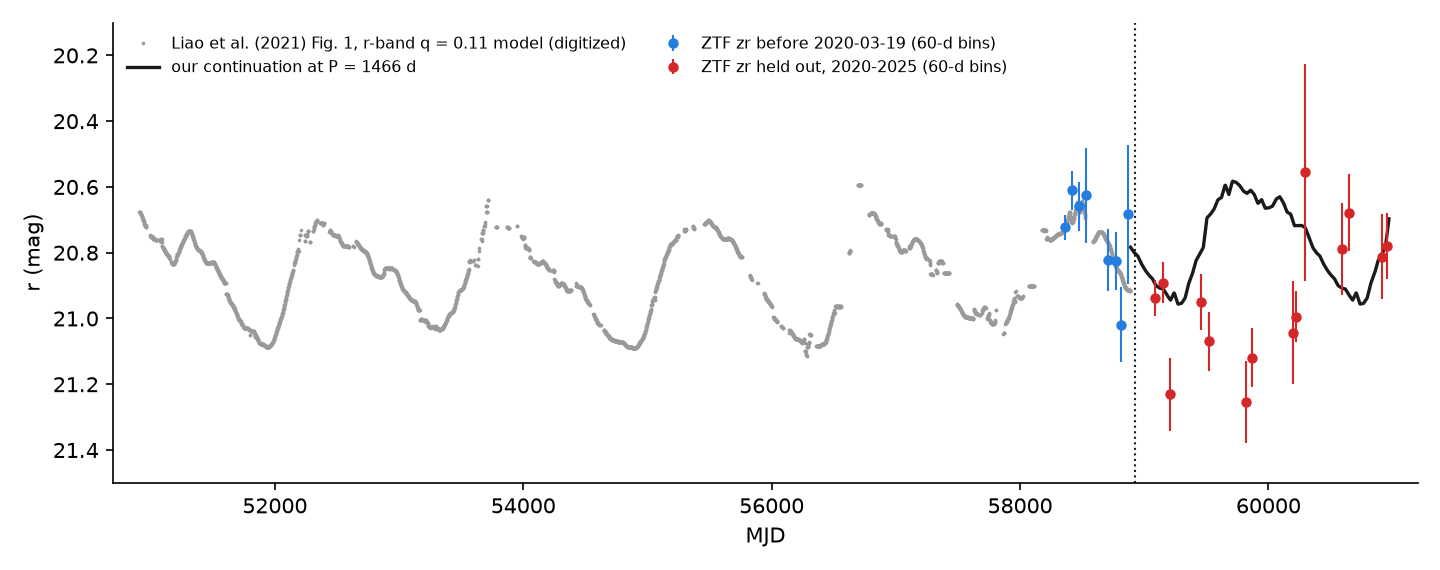
\includegraphics[width=\textwidth]{fig_forecast.png}
\caption{Grey: the digitized r-band model of Liao et al.\ (their Figure~1). Black: our continuation at $P = 1466$~d. Points: ZTF zr detections in 60-day bins, before (blue) and after (red) the cutoff (dotted line). Each ZTF object is shifted to the median of the model curve over MJD 58300--58889. Near the detection limit the listed points are biased bright, so the binned points are a guide only. The test uses the unbinned points.}
\label{fig:forecast}
\end{figure}

\subsection{The observed statistic}
The held-out data give $\Tobs = -0.664$ (Figure~\ref{fig:forecast}). The data are faint where the continuation predicts the broad maximum near MJD 59800--60200. A phase scan of the template in steps of 0.05 cycles puts the predicted phase at rank 19 of 20. The largest $T$ (1.03) is at a shift of 0.55 cycles. $T$ stays negative when we add the limiting magnitude as a covariate ($T = -0.53$), when we use only the 53 points from exposures with $L > 21.3$ ($T = -0.57$), and when we build the template from the last cycle of the model curve only ($T = -0.91$). The listed magnitudes correlate with the limiting magnitude (correlation 0.69, slope 0.57). The zg band (34 points, descriptive only) gives $T = -0.12$.

As a positive control, the 72 ZTF zr points before the cutoff (2018-07 to 2020-03, about 600~d) give $T = +1.72$. Liao et al.\ plotted these ZTF points in their Figure~1, and their model was fitted to data that include this window. So this control shows only that the time and magnitude axes of the digitization are not inverted or shifted by a large amount. It does not show that the template is correct.

\subsection{Original protocol}
Under the registered noise model (DRW rms 0.119~mag), $\pnull = 0.949$ and $\psig < 2\times10^{-4}$ (0 of 5000 mocks); the power is 0.59. By the registered rule this is a refutation. The verification showed that the noise model omits the detection limit: under censoring, the median $T$ of signal mocks is about 0.6, not 1. So we do not use this decision. We keep the numbers for the record.

\subsection{Censored model (Addendum 1)}
Table~\ref{tab:censored} gives the main results. At the best-fit DRW of Liao et al., the censored mocks give a median $T$ of 0.61 if the forecast is true, with a standard deviation of 0.36. Then $\Tobs = -0.66$ gives $\psig = 0.0005$ and $\pnull = 0.965$. The power to detect the forecast at $\pnull < 0.01$ is about 0.3.

\begin{table}[t]
\centering
\caption{Censored forward model. $\psig$: probability of $T \le -0.664$ if the forecast is true. $\pnull$: probability of $T \ge -0.664$ if there is no relation. Power: fraction of $a = 1$ mocks with $\pnull < 0.01$. 4000 mocks per row, 2000 per contour point. The text gives the power to one digit because the 99\% null quantile is noisy.}
\label{tab:censored}
\begin{tabular}{lcccc}
\toprule
DRW parameters & $\psig$ & $\pnull$ & median $T$ ($a=1$) & power \\
\midrule
best fit ($\tau = 794$~d, $\sigma = 0.15$) & 0.0005 & 0.965 & 0.61 & 0.30 \\
$\tau = 716$~d, $\sigma = 0.10$ & 0 & 0.99 & 0.64 & 0.59 \\
$\tau = 716$~d, $\sigma = 0.119$ & 0 & 0.98 & 0.62 & 0.46 \\
$\tau = 716$~d, $\sigma = 0.13$ & 0 & 0.97 & 0.61 & 0.44 \\
$\tau = 716$~d, $\sigma = 0.15$ & 0.0005 & 0.96 & 0.62 & 0.30 \\
$\tau = 716$~d, $\sigma = 0.17$ & 0.0008 & 0.94 & 0.58 & 0.28 \\
$\tau = 716$~d, $\sigma = 0.20$ & 0.0048 & 0.93 & 0.59 & 0.18 \\
$\tau = 716$~d, $\sigma = 0.25$ & 0.017 & 0.88 & 0.54 & 0.11 \\
$\tau = 716$~d, $\sigma = 0.30$ & 0.031 & 0.83 & 0.50 & 0.09 \\
68\% contour, 12 points & max 0.002 & & 0.56--0.63 & 0.23--0.45 \\
95\% contour, 24 points (plotted part) & max 0.035 & & 0.50--0.64 & 0.03--0.46 \\
\bottomrule
\end{tabular}
\end{table}

Without the inflation, $\psig < 0.01$ on the whole 68\% contour. On the 95\% contour, $\psig \ge 0.01$ only at the long-$\tau$, large-$\sigma$ end ($\tau \gtrsim 10^{3.48}$~d and $\sigma \ge 0.33$~mag; 5 of 24 points; Figure~\ref{fig:drw}). The plotted 95\% contour of Liao et al.\ reaches the edge of the axes near $\log_{10}\tau = 3.85$ and $\sigma = 0.47$. The true 95\% region can extend beyond this edge, so the value 0.035 is the maximum on the plotted part only. At $\tau = 716$~d the 95\% contour spans $\sigma = 0.117$ to 0.177, and $\psig$ crosses 0.01 between $\sigma = 0.20$ and 0.25.

\begin{figure}[t]
\centering
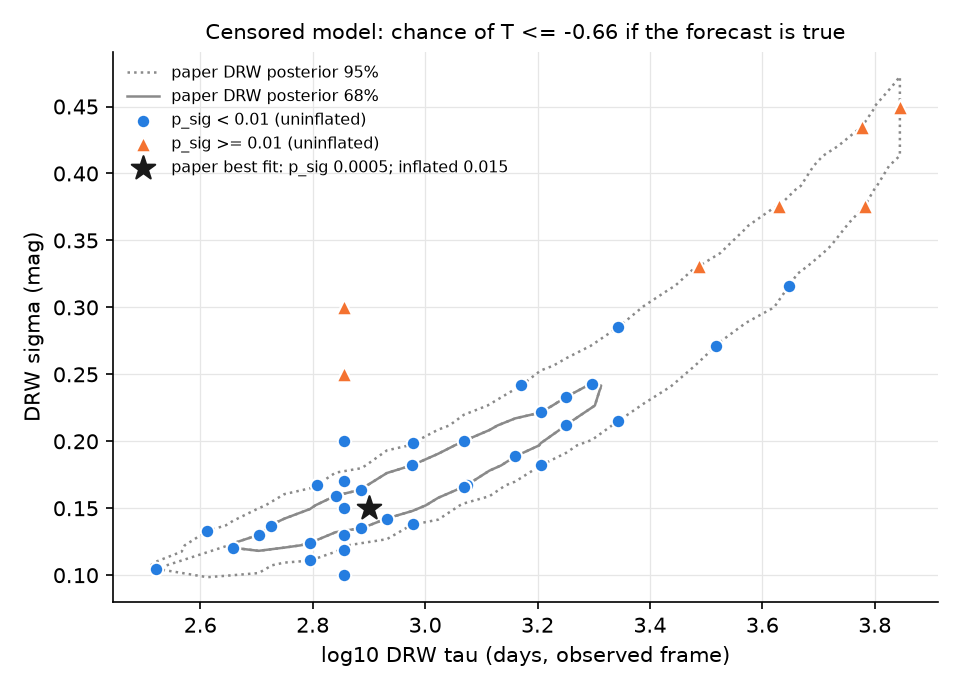
\includegraphics[width=0.68\textwidth]{fig_addendum.png}
\caption{$\psig$ of the censored model, without inflation, across the published r-band DRW posterior of Liao et al.\ (68\% solid, 95\% dotted, as plotted in their figure). Circles: $\psig < 0.01$. Triangles: $\psig \ge 0.01$. Star: their best fit.}
\label{fig:drw}
\end{figure}

\subsection{Model checks and calibration}
The censored mocks reproduce the dependence on depth. The slope of magnitude against limiting magnitude is 0.62 in the mocks (median) and 0.57 in the data. The listed fraction in five bins of limiting magnitude ($<20.5$, 20.5--21, 21--21.3, 21.3--21.6, $>21.6$) is 0.03, 0.14, 0.43, 0.63, 0.65 in the data and 0.01, 0.10, 0.40, 0.66, 0.92 in the mocks. The deepest bin has 23 exposures, and the quasar is listed on 15. The mocks overpredict this fraction. We did not find the cause.

The placebo objects show more scatter in $T$ than the model gives. Their $z$ values have a median of $-0.01$, a robust standard deviation of 1.67 and a standard deviation of 2.07. So the data contain slow, time-correlated errors that the model lacks. $|z|$ does not correlate with the absolute value of the median PSF sharpness of the objects (Spearman $-0.12$, $p = 0.38$), so extended sources do not explain the excess. One of the 51 placebo objects has $T \le \Tobs$.

The registered rule (robust standard deviation above 1.2) applies. With the factor 1.67, $\psig = 0.015$ at the best fit. The factor is not a sharp number, and Table~\ref{tab:calib} lists the alternatives. All calibrated values are 0.01 to 0.04. All are above the threshold of 0.01.

\begin{table}[t]
\centering
\caption{$\psig$ at the best-fit DRW for different calibrations of the excess scatter. Rows marked ``indep.'' come from the independent implementation of the verification stage (\texttt{checks/verify/v4\_censored\_independent.py}), with other random seeds. Rows marked post hoc were not in the addendum.}
\label{tab:calib}
\begin{tabular}{lc}
\toprule
Calibration & $\psig$ \\
\midrule
none & 0.0005 \\
whole $T$ scatter $\times 1.67$ (registered rule, our mocks) & 0.015 \\
whole $T$ scatter $\times 1.67$ (indep.) & 0.0175 \\
whole $T$ scatter $\times 2.07$ (plain standard deviation of $z$; indep.) & 0.043 \\
DRW part plus raw $T$ scatter of 25 placebo objects (indep., post hoc) & 0.0105 \\
white-noise part only $\times 1.67$ (post hoc) & 0.0015 \\
\bottomrule
\end{tabular}
\end{table}

\subsection{Decision}
The registered rule of Addendum~1 uses the inflated $\psig$. It is 0.015 at the best fit, and every other calibration of the excess scatter gives 0.01 to 0.04. All of these are $\ge 0.01$, so the decision is \emph{not refuted}. Without a threshold, the data disfavour the continuation: no check detects the predicted signal ($\pnull = 0.965$), and $T$ is negative in every variant. But the power is only about 0.3, so the data could not have confirmed the forecast either.

\subsection{Other periods (post hoc)}\label{sec:scope}
Table~\ref{tab:periods} gives the censored model at the best-fit DRW, without inflation, for the other periods of Table~2 of Liao et al. The periods of the r, i, g and joint fits all give negative $T$. The two periods near the Lomb--Scargle value give positive $T$ and $\pnull \approx 0.05$. The 1604~d value is the upper 1-$\sigma$ end of the joint fit; 1607~d is the g-band Lomb--Scargle period. So the data do not exclude a continuation of the 4.4-yr periodicity near 1600~d. These rows were chosen after the result of the main test was known. They are descriptive.

\begin{table}[t]
\centering
\caption{Other periods of Liao et al.\ (Table~2), censored model at the best-fit DRW, no inflation, 2000 mocks. Post hoc.}
\label{tab:periods}
\begin{tabular}{lcccccccc}
\toprule
$P$ (d) & 1454 & 1476 & 1506 & 1511 & 1530 & 1562 & 1604 & 1607 \\
 & r low & joint & i & g & r high & z & joint high & GLS \\
\midrule
$\Tobs$ & $-0.51$ & $-0.78$ & $-0.65$ & $-0.61$ & $-0.49$ & $-0.24$ & $+0.93$ & $+1.12$ \\
$\psig$ & 0 & 0 & 0.0005 & 0.0005 & 0 & 0.0075 & 0.56 & 0.65 \\
$\pnull$ & 0.94 & 0.97 & 0.98 & 0.97 & 0.96 & 0.83 & 0.054 & 0.058 \\
\bottomrule
\end{tabular}
\end{table}

\section{How the result was checked}
\begin{itemize}
\item \textbf{Order of commits.} The protocol (commit \texttt{f6a2c6d}) precedes the first comparison (\texttt{5f19203}). Addendum~1 (\texttt{a7f1e6f}) precedes the censored computation (\texttt{01a9e44}). The commit order is the only evidence that no result was seen before each protocol commit.
\item \textbf{Reruns from a clean clone.} A separate verification session cloned the repository twice, downloaded the data again from IRSA and reran \texttt{checks/rerun.py}. Both runs printed \texttt{OK}: every number matched \texttt{data/expected.json}. The figure and the DRW-contour digitization were reproduced byte for byte. The digitizer of the model curve gave identical output on a new download of the arXiv source.
\item \textbf{Independent implementation.} The verification session wrote its own censored model from the text of the addendum, without the code of \texttt{checks/censored.py}. It reproduced the 345 exposures, the 97 listed points, $k = 1.416$ and $\Tobs = -0.6636$. With other seeds it gave $\psig = 0.0005$, median $T$ 0.61, a robust placebo scatter of 1.75 and an inflated $\psig$ of 0.0175 (Table~\ref{tab:calib}).
\item \textbf{Quotes.} The quotes of Liao et al.\ were compared with the arXiv source. The DRW labels were read from the PDF with \texttt{pymupdf}.
\item \textbf{This release.} \texttt{checks/ci.sh} reruns the full computation from the public data and fails on any difference from \texttt{data/expected.json}. We ran it from a clean copy with a new Python environment (see \texttt{NUMBERS.md}).
\end{itemize}

\section{Limits}
\begin{itemize}
\item The forecast is our construction. Liao et al.\ give no forecast. The template comes from a digitized raster figure, and the model curve is not strictly periodic.
\item The censored model is simple: sky-limited flux noise, a sharp cut at $S/N = 4$, no seeing or calibration terms. The placebo shows slow errors that it lacks. The inflation factor comes from 51 objects, and some of them can be variable.
\item The DRW posterior of Liao et al.\ is from a DRW-only fit, so it includes the variance of the periodic signal. Under ``model plus DRW'' the DRW amplitude would be smaller, and $\psig$ would be smaller. We did not model this.
\item Near the detection limit the ZTF magnitudes are biased bright. The model reproduces this in kind but overpredicts the listed fraction in the deepest bin.
\item One object, two ZTF fields, five years: about 1.3 cycles of the continuation. The power is about 0.3.
\item The positive control uses ZTF data that Liao et al.\ plotted. It is a weak check.
\end{itemize}
Forced photometry at the quasar position, from the ZTF forced-photometry service or from deeper images, would give a flux at every exposure with no detection cut. Such data would raise the power and could settle the continuation.

\section{Prior-art search}\label{sec:prior}
On 2026-11-28 we read the titles of the 48 works in OpenAlex that cite Liao et al.\ and of the 90 works that cite Chen et al.\ (2020). Only Foord et al.\ (2022) and Covino et al.\ (2022) study J0252, and neither uses data after 2020. Among the 19 works that cite Covino et al., Gúrpide and Middleton (2025) \cite{gurpide2025} develop periodicity methods for unevenly sampled data. Their applications do not include J0252 or ZTF. We also searched two public collections of AI-produced results, issue trackers where such groups post results, Zenodo and the web. We found no forward test of J0252 on post-2020 data. Liao et al.\ wrote that follow-up with DECam was on-going \cite{liao2021}; we found no published result from it. On 2026-11-28 the recheck stage repeated the archive searches, the OpenAlex citation lists of both papers (sorted by date) and two web searches. It found no new work on J0252.

\section*{Data and code}
All data are public and need no account. \texttt{checks/rerun.py} downloads the ZTF light curves from IRSA and reproduces every number in this paper. The result folder lists the data sources, their terms and the access dates (\texttt{THIRD\_PARTY.md}), and the source of each number (\texttt{NUMBERS.md}). This work uses data from the Zwicky Transient Facility and the NASA/IPAC Infrared Science Archive.

\begin{thebibliography}{99}
\bibitem{bellm2019} E.~C. Bellm et al., The Zwicky Transient Facility: system overview, performance, and first results, PASP 131, 018002 (2019), \href{https://doi.org/10.1088/1538-3873/aaecbe}{doi:10.1088/1538-3873/aaecbe}.
\bibitem{chen2020} Y.-C. Chen, X. Liu, W.-T. Liao et al., Candidate periodically variable quasars from the Dark Energy Survey and the Sloan Digital Sky Survey, MNRAS 499, 2245 (2020), \href{https://doi.org/10.1093/mnras/staa2957}{doi:10.1093/mnras/staa2957}.
\bibitem{chen2024} Y.-J. Chen, S. Zhai, J.-R. Liu et al., Searching for quasar candidates with periodic variations from the Zwicky Transient Facility: results and implications, MNRAS 527, 12154 (2024), \href{https://doi.org/10.1093/mnras/stad3981}{doi:10.1093/mnras/stad3981}.
\bibitem{covino2022} S. Covino, F. Tobar, A. Treves, Detecting the periodicity of highly irregularly sampled light curves with Gaussian processes: the case of SDSS J025214.67$-$002813.7, MNRAS 513, 2841 (2022), \href{https://doi.org/10.1093/mnras/stac596}{doi:10.1093/mnras/stac596}.
\bibitem{elbadry2026} K. El-Badry, D.~W. Hogg, H.-W. Rix, Active galactic nuclei do not exhibit strictly sinusoidal brightness variations, PASP 138, 024102 (2026), \href{https://doi.org/10.1088/1538-3873/ae3f56}{doi:10.1088/1538-3873/ae3f56}.
\bibitem{foord2022} A. Foord, X. Liu, K. G\"ultekin et al., Investigating the accretion nature of binary supermassive black hole candidate SDSS J025214.67$-$002813.7, ApJ 927, 3 (2022), \href{https://doi.org/10.3847/1538-4357/ac4af1}{doi:10.3847/1538-4357/ac4af1}.
\bibitem{gurpide2025} A. G\'urpide, M. Middleton, Mind the gaps: improved methods for the detection of periodicities in unevenly sampled data, MNRAS 537, 3210 (2025), \href{https://doi.org/10.1093/mnras/staf196}{doi:10.1093/mnras/staf196}.
\bibitem{kelly2009} B.~C. Kelly, J. Bechtold, A. Siemiginowska, Are the variations in quasar optical flux driven by thermal fluctuations?, ApJ 698, 895 (2009), \href{https://doi.org/10.1088/0004-637X/698/1/895}{doi:10.1088/0004-637X/698/1/895}.
\bibitem{liao2021} W.-T. Liao, Y.-C. Chen, X. Liu et al., Discovery of a candidate binary supermassive black hole in a periodic quasar from circumbinary accretion variability, MNRAS 500, 4025 (2021), \href{https://doi.org/10.1093/mnras/staa3055}{doi:10.1093/mnras/staa3055}, arXiv:2008.12317.
\bibitem{masci2019} F.~J. Masci et al., The Zwicky Transient Facility: data processing, products, and archive, PASP 131, 018003 (2019), \href{https://doi.org/10.1088/1538-3873/aae8ac}{doi:10.1088/1538-3873/aae8ac}.
\bibitem{rigamonti2025} F. Rigamonti, L. Bertassi, R. Buscicchio et al., Variability in the supermassive black hole binary candidate SDSS J2320+0024: no evidence of periodic modulation, A\&A 702, A242 (2025), \href{https://doi.org/10.1051/0004-6361/202555550}{doi:10.1051/0004-6361/202555550}.
\bibitem{vaughan2016} S. Vaughan, P. Uttley, A.~G. Markowitz et al., False periodicities in quasar time-domain surveys, MNRAS 461, 3145 (2016), \href{https://doi.org/10.1093/mnras/stw1412}{doi:10.1093/mnras/stw1412}.
\bibitem{wu2026} Q. Wu, A pre-registered forward test of 86 ZTF periodic-quasar candidates finds no predictive periodicity (2026), \href{https://doi.org/10.5281/zenodo.24580702}{doi:10.5281/zenodo.24580702}.
\end{thebibliography}
\end{document}
